
\cellname{FULLADDER}
\designer{Martin Wearn}
\celldescription{Adds two bit values and the previous bitsclie carry out, to produce a sum and carry}
%\topimages{../fulladder/symbol.png}{../fulladder/circuitdiagram.pdf}{../fulladder/blackbox.pdf}

%\acchar{../fulladder/acresults.txt}

%\sysverilog{../fulladder/sv.pdf}


%manual override

\begin{figure}[ht!]
        \centering
        \begin{subfigure}[b]{0.5\textwidth}
			\subsection*{Symbol}
                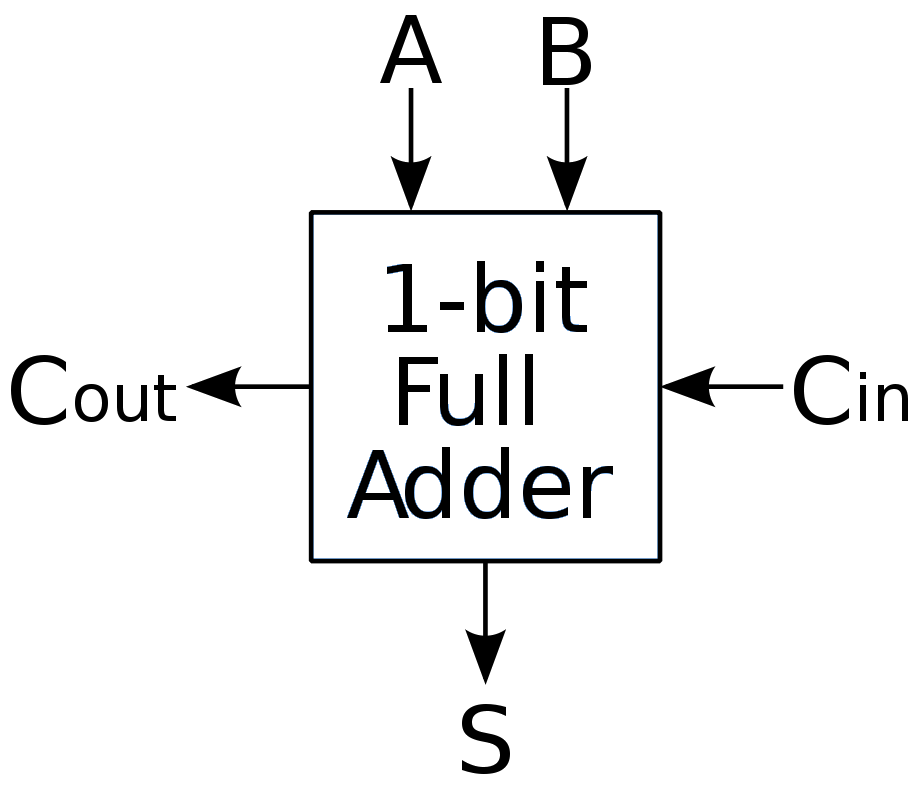
\includegraphics[width=\textwidth,height=4cm,keepaspectratio]{../fulladder/symbol.png}
        \end{subfigure}%
        ~ %add desired spacing between images, e. g. ~, \quad, \qquad etc.
          %(or a blank line to force the subfigure onto a new line)
        \begin{subfigure}[b]{0.5\textwidth}
				\subsection*{Dimensions}
                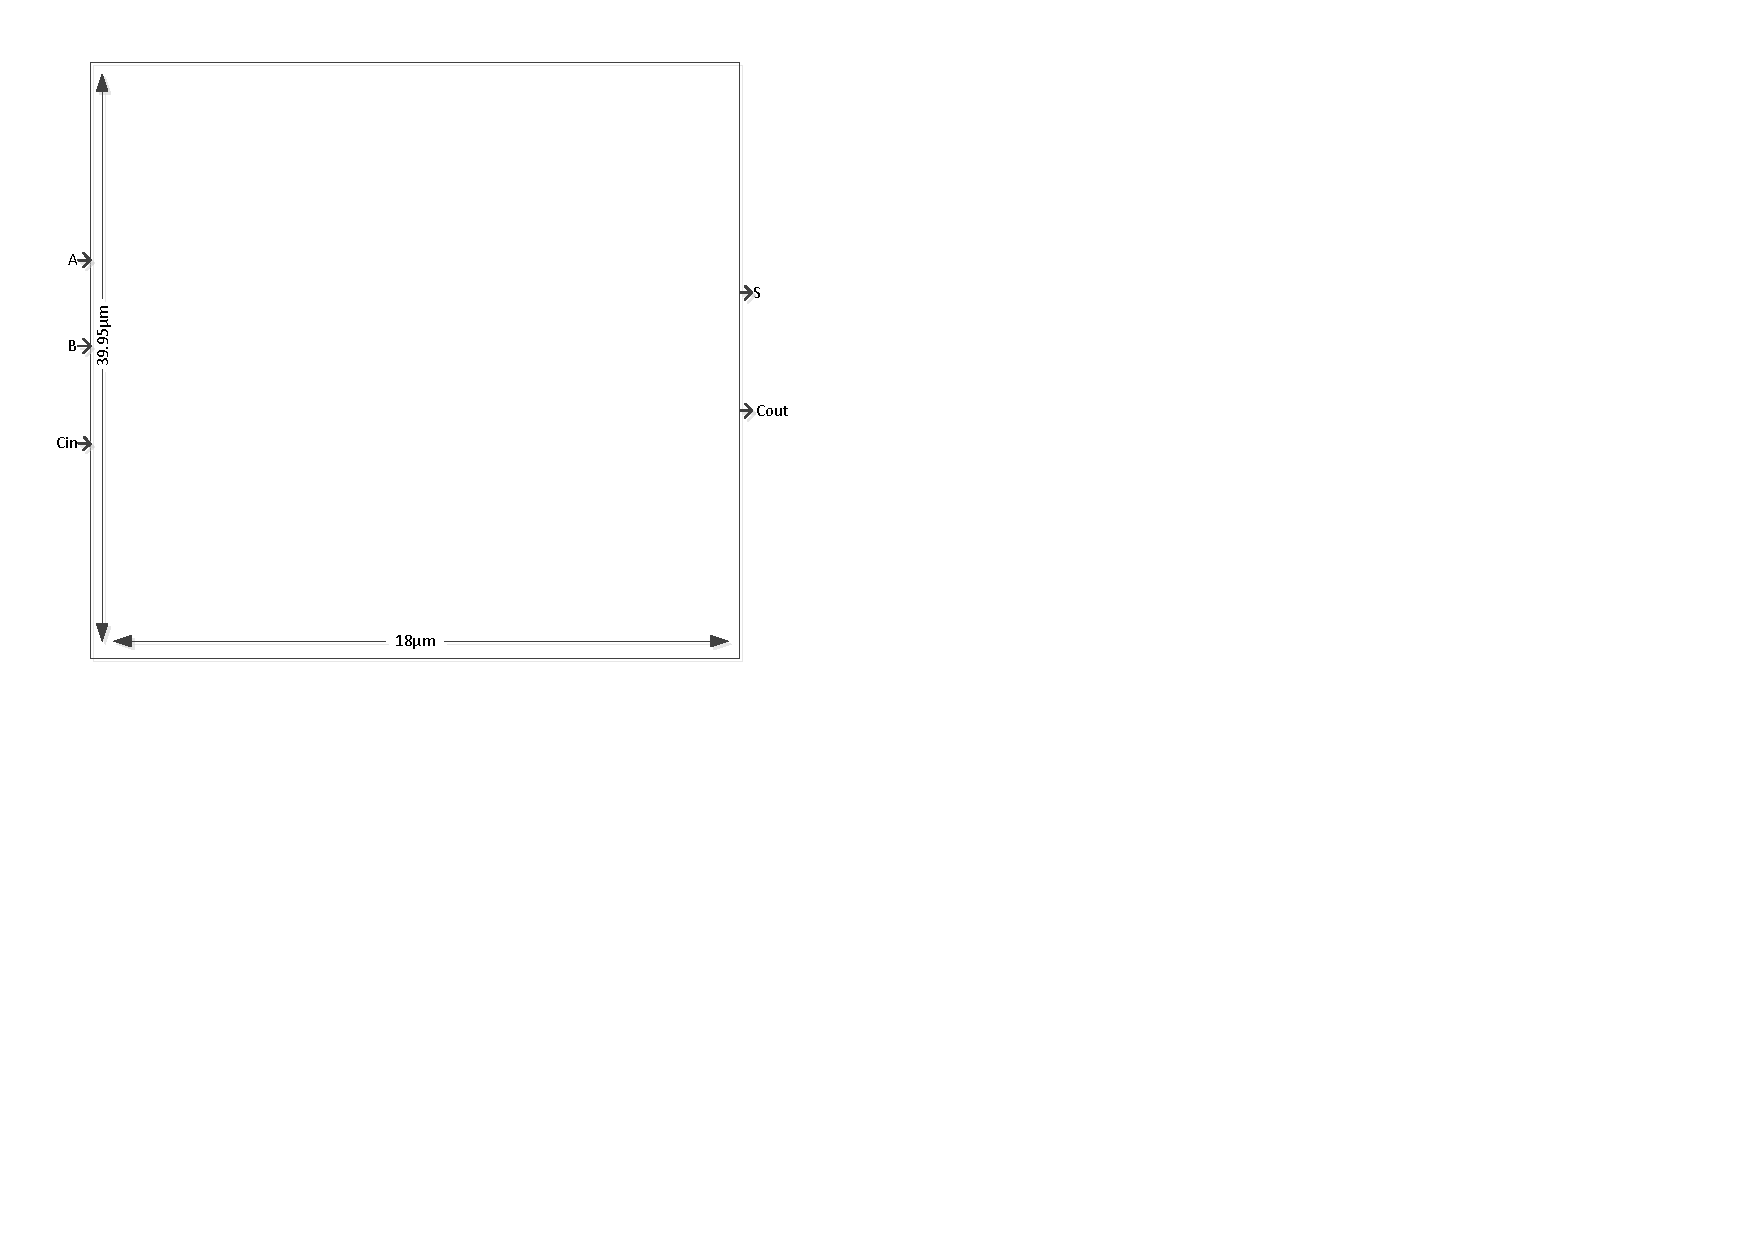
\includegraphics[width=\textwidth,height=4cm,keepaspectratio]{../fulladder/blackbox.pdf}
        \end{subfigure}
		~ %add desired spacing between images, e. g. ~, \quad, \qquad etc.
          %(or a blank line to force the subfigure onto a new line)
        \begin{subfigure}[b]{0.7\textwidth}
				\subsection*{Gate Level Diagram}
                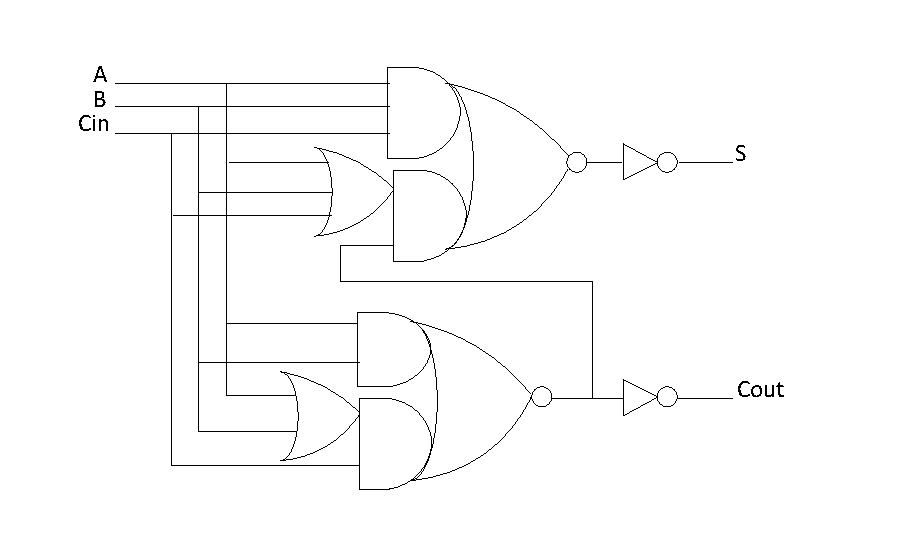
\includegraphics[width=\textwidth,height=4cm,keepaspectratio]{../fulladder/circuitdiagram.pdf}
        \end{subfigure}
\end{figure}



\subsection*{AC Characteristics}
\begin{table}[h!]
\centering
\begin{tabular}{cc}
Signal & Average Delay (ps) \\ \hline
\input{../fulladder/acresults.txt} 
\end{tabular}
\end{table}

\subsection*{System Verilog Simulation} 
\begin{figure}[h!] 
\centering 
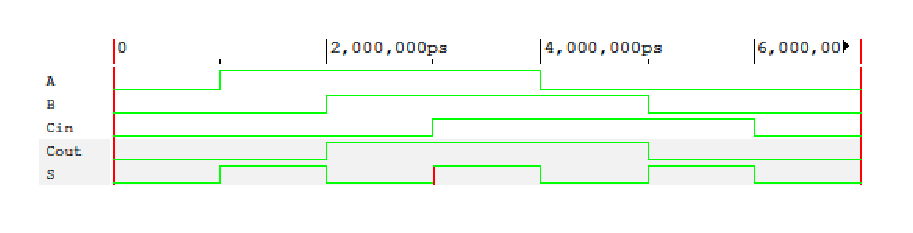
\includegraphics[width=\textwidth]{../fulladder/sv.pdf} 
\end{figure}